\subsection{JetFitter}
\label{subsec:jf}

\begin{itemize}
	\item Motivation for JF: Cascade topology
	\item Key assumption: Every (well motivated b/c the B-hadron caries a large portion of the initial quarks momentum which causes the B (and subsequent D) hadrons to form a line with respect to the
	\item Briefly sketch the extension to the KF formalism
	\item The track selection and JF algorithm
	\item The final variables defining the JF algorithm and variables targetting \Pqc-tagging
	\item Mass constraint
\end{itemize}

\begin{figure}
\centering
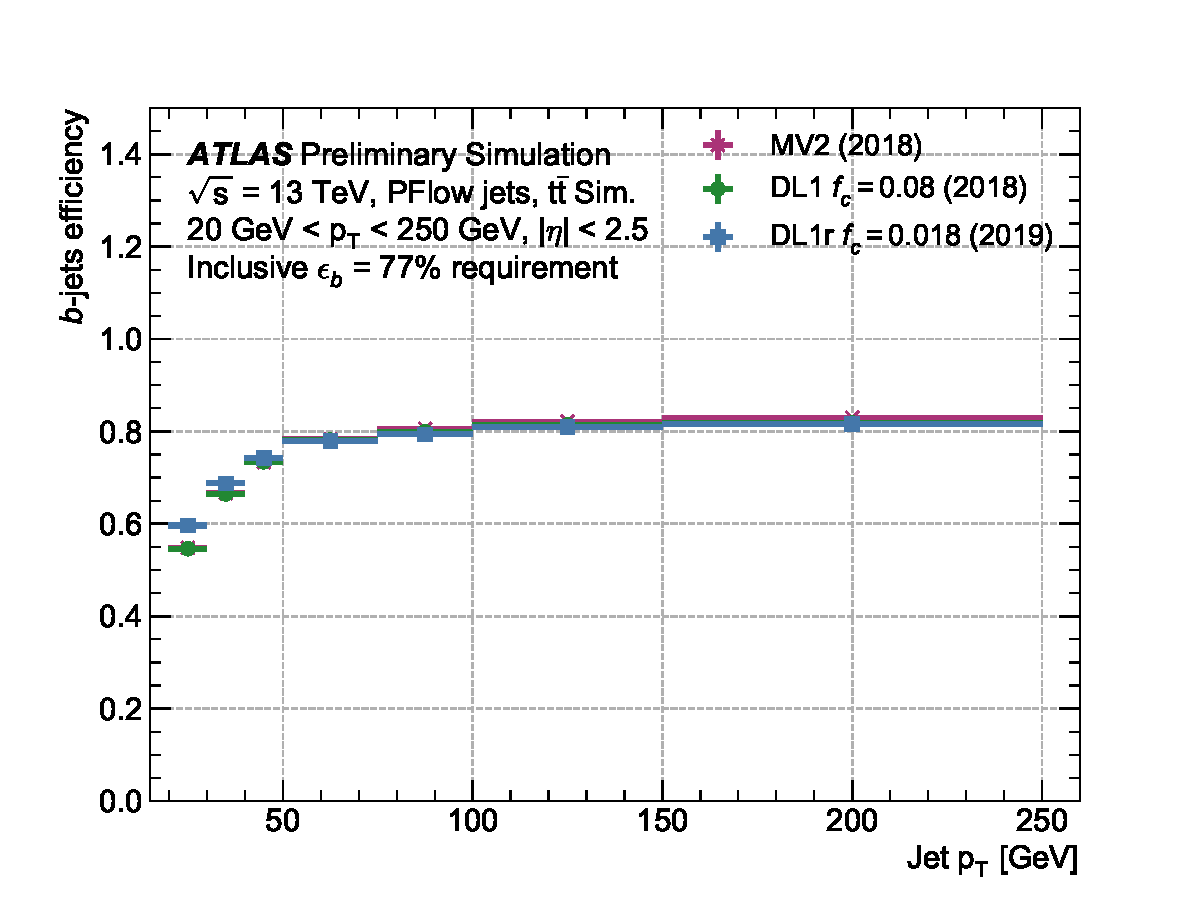
\includegraphics[width=.6\textwidth]{{figures/ftag/ATL-PHYS-PUB-2018-025/fig_02a.pdf}} 
% Note fig (b) shows the reconstruction level picture
\caption{\cite{ATL-PHYS-PUB-2018-025}}
\label{fig:jf-fig-02a}
\end{figure}

\textbf{Mass constraints}

\hl{I should note the motivation for these checks?}

\begin{minipage}{0.6\textwidth}
\begin{itemize}
	\item \textcolor{blue}{$p$}	: 4-vector of the \textcolor{blue}{charged} particles
	\item \textcolor{red}{$q$}: 4-vector for \textcolor{red}{neutral} particles
	\item Let $p_{true} = p + q$ be the true 4-vector of charged and neutral particles. 
\end{itemize}

\hspace{0.03\textwidth}
\end{minipage}
\begin{minipage}{0.35\textwidth}
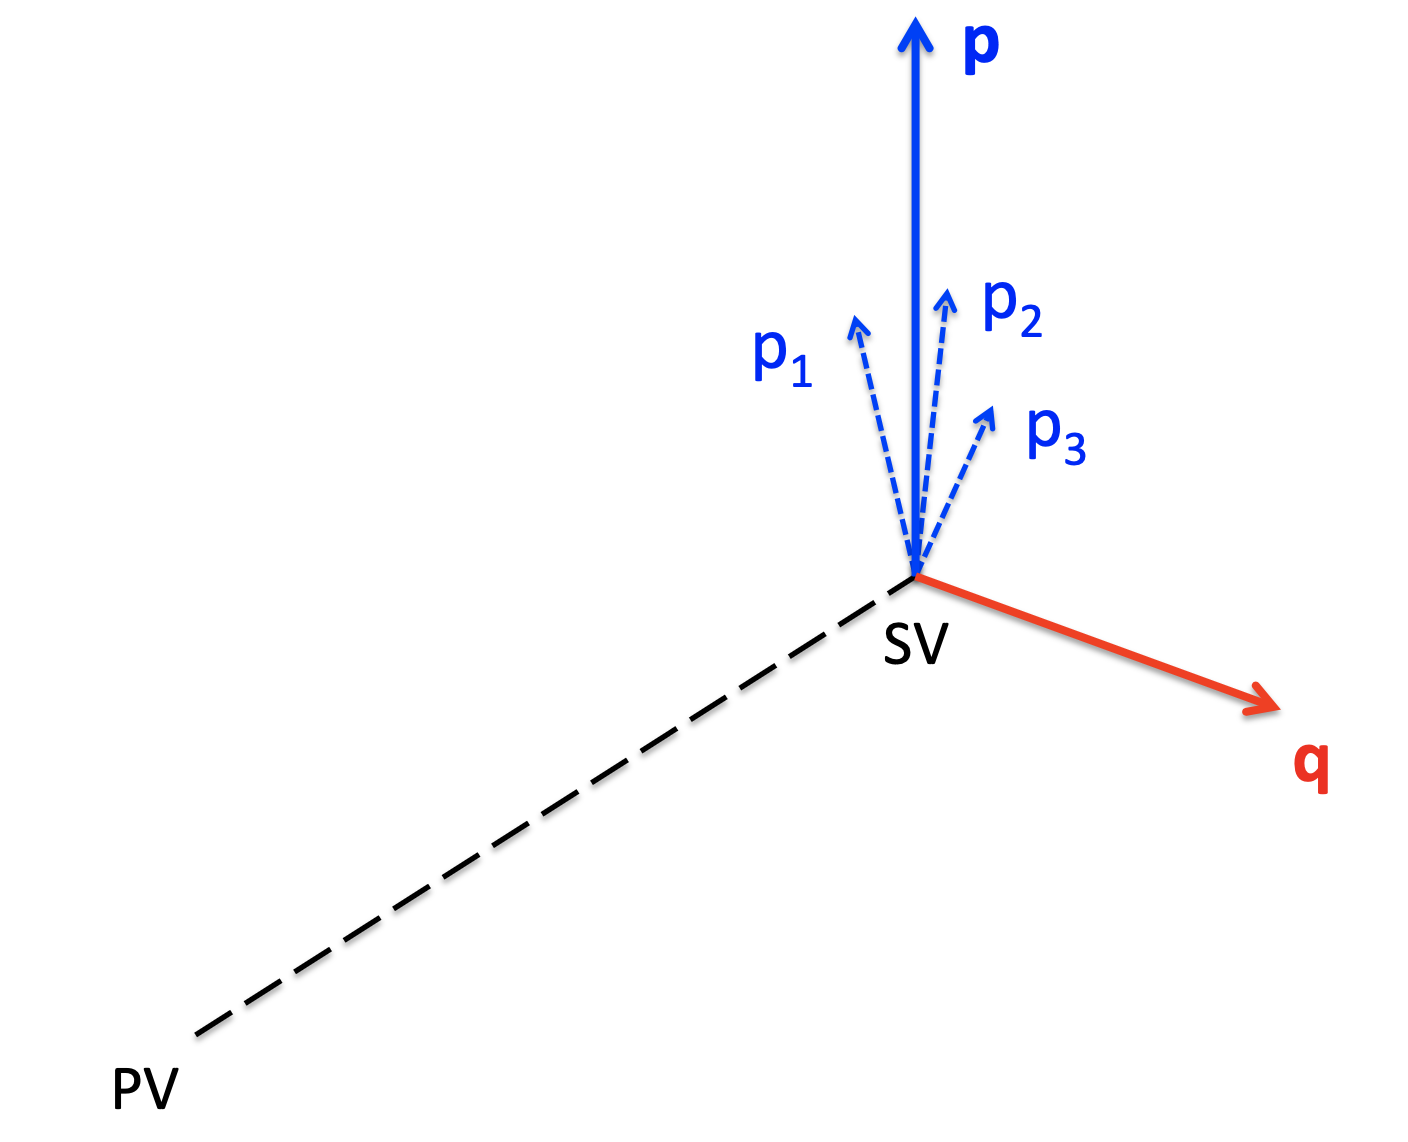
\includegraphics[width=\textwidth]{figures/ftag/mass-regression/mass-pt-constraint}
\end{minipage}

Then $p = p_{true} -q$, which we can then square. We additionally make a simplifying assumption that the neutral particles are massless:
\begin{equation}
p^2 = p_{true}^2 - 2 p \cdot q + \cancelto{0}{q^2}
\label{eq:chg-neutral}
\end{equation}

Let $p^2 = m_{ch}^2$ the mass from the charged particles, and $p_{true}^2 = m^2$, the weakly decaying hadron mass. 
Then evaluate the right hand side of \Eq{\ref{eq:chg-neutral}} in the hadron's rest frame ($\vec{p}_{true}^{CM} = 0$).  Then \textcolor{red}{$q$} is perpendicular to the hadron's flight axis $|\vec{q}^{CM}| = q_\perp$, where the ``CM'' superscript denotes the hadron's center-of-mass frame, and $q_\perp$ is the component of $\vec{q}$ perpendicular to the hadron's flight axis, which is invariant to boosts along the flight axis.

\begin{equation}
m_{ch}^2 = m^2 - 2 \left( m q_\perp - \cancelto{0}{\vec{p}_{true}^{CM}} \cdot \vec{q}^{CM} \right)
\end{equation}

\begin{equation}
m_{ch}^2 + p_\perp^2 = m^2 - 2 m p_\perp + p_\perp^2 = (m - p_\perp^2)^2
\end{equation}

and solve for $m$:

\begin{equation}
m = \sqrt{m_{ch}^2 + p_\perp^2} + p_\perp
\label{eq:mass-neutrals}
\end{equation}

where we took the $+$ solution of the $\sqrt{ \ }$ for the physical solution of the positive hadron mass.

\begin{figure}
\centering
\subfloat[$B$-hadron reconstruction]{
	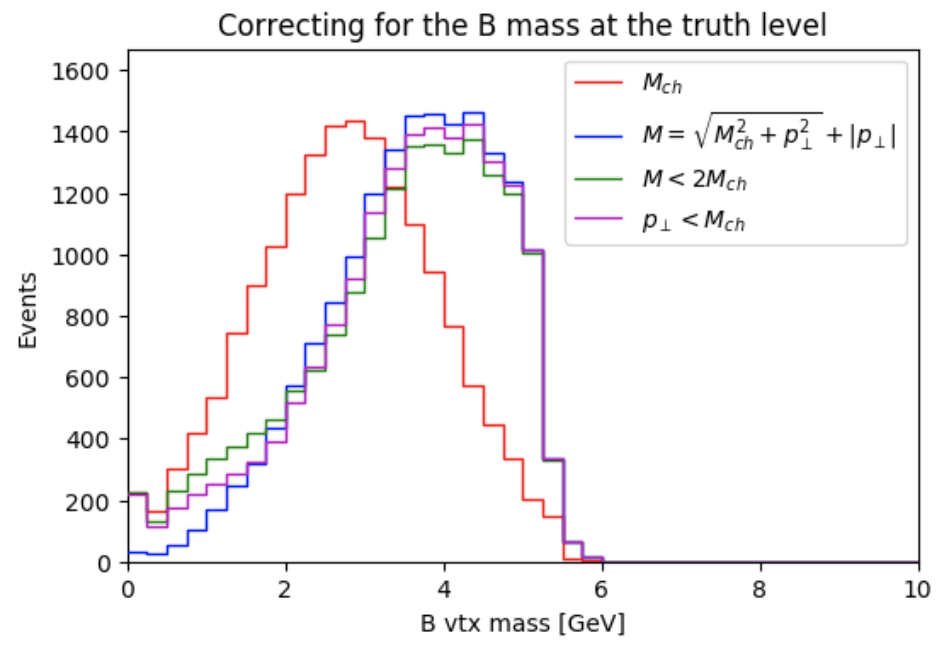
\includegraphics[width=0.45\textwidth]{{figures/ftag/mass-regression/truth-b-had-mass.png}}
	}
\subfloat[$D$-hadron reconstruction]{
	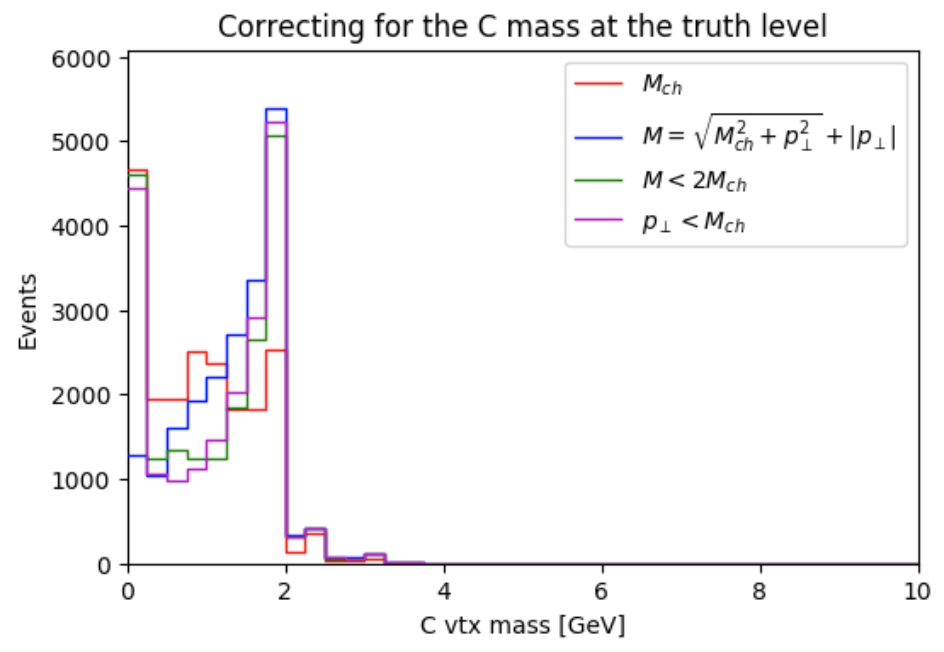
\includegraphics[width=0.45\textwidth]{{figures/ftag/mass-regression/truth-c-had-mass.png}}
	}
\caption{Reconstruction of the $B$ (left) and $D$ (right) hadron masses from the truth charged particles.}
\label{fig:truth-had}
\end{figure}


How JF applies the mass correction:
\begin{itemize}
	\item It uses the scalar sum of the tracks, $p = \sum_i p_\perp^{(i)}$, where $i$ runs over the tracks in the jet. Then just replace the vector sum over the tracks with the scalar sum over the tracks in the formula as: $m= \sqrt{m_{ch}^2 +p_\perp^2} +|p_\perp|$.
	\item To constrain the tails, if $m > 5$, $m \leftarrow 5\left[1 + 2 \arctan( \pi (m - 5) )\right]$.
\end{itemize}

\begin{figure}%[hbt]
\centering
\subfloat[Vertex reco in \Pqb-jets]{
	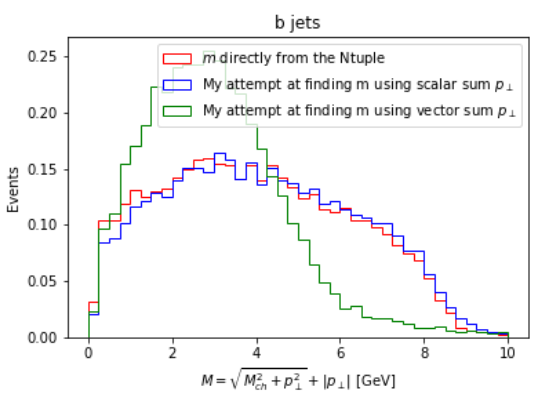
\includegraphics[width=0.33\textwidth]{{figures/ftag/mass-regression/b-had-jf-mass}}
	}
\subfloat[Vertex reco in \Pqc-jets]{
	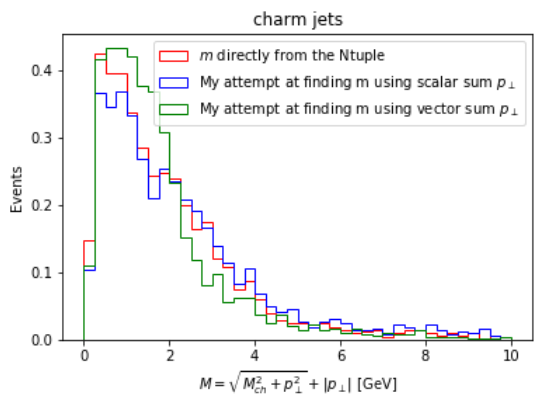
\includegraphics[width=0.33\textwidth]{{figures/ftag/mass-regression/c-had-jf-mass}}
	} 
\subfloat[Vertex reco in light jets]{
	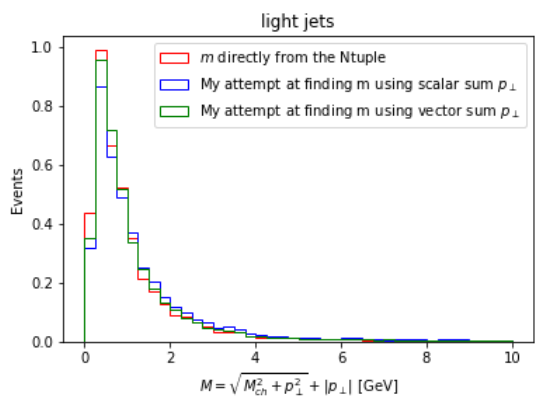
\includegraphics[width=0.33\textwidth]{{figures/ftag/mass-regression/l-reco-jf-mass}}
}
\caption{}%Reconstruction of the $B$ (left) and $D$ (right) hadron masses from the truth charged particles.}
\label{fig:jf-reco-mass}
\end{figure}


\begin{figure}%[hbt]
\centering
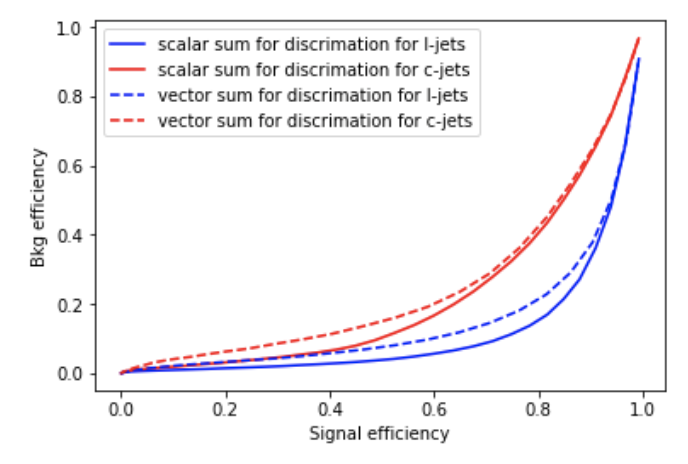
\includegraphics[width=0.7\textwidth]{{figures/ftag/mass-regression/roc-jf-mass-scalar-vs-vector}}
\caption{}%Reconstruction of the $B$ (left) and $D$ (right) hadron masses from the truth charged particles.}
\label{fig:jf-reco-mass-roc}
\end{figure}

As more tracks are dropped, the scalar sum does increasingly better over the vector sum.
Mean number of truth particles not reconstructed:  0.88
Mean truth particles not found by JetFitter:  2.15

\begin{figure}%[hbt]
\centering
\subfloat[$B$-hadron reconstruction]{
	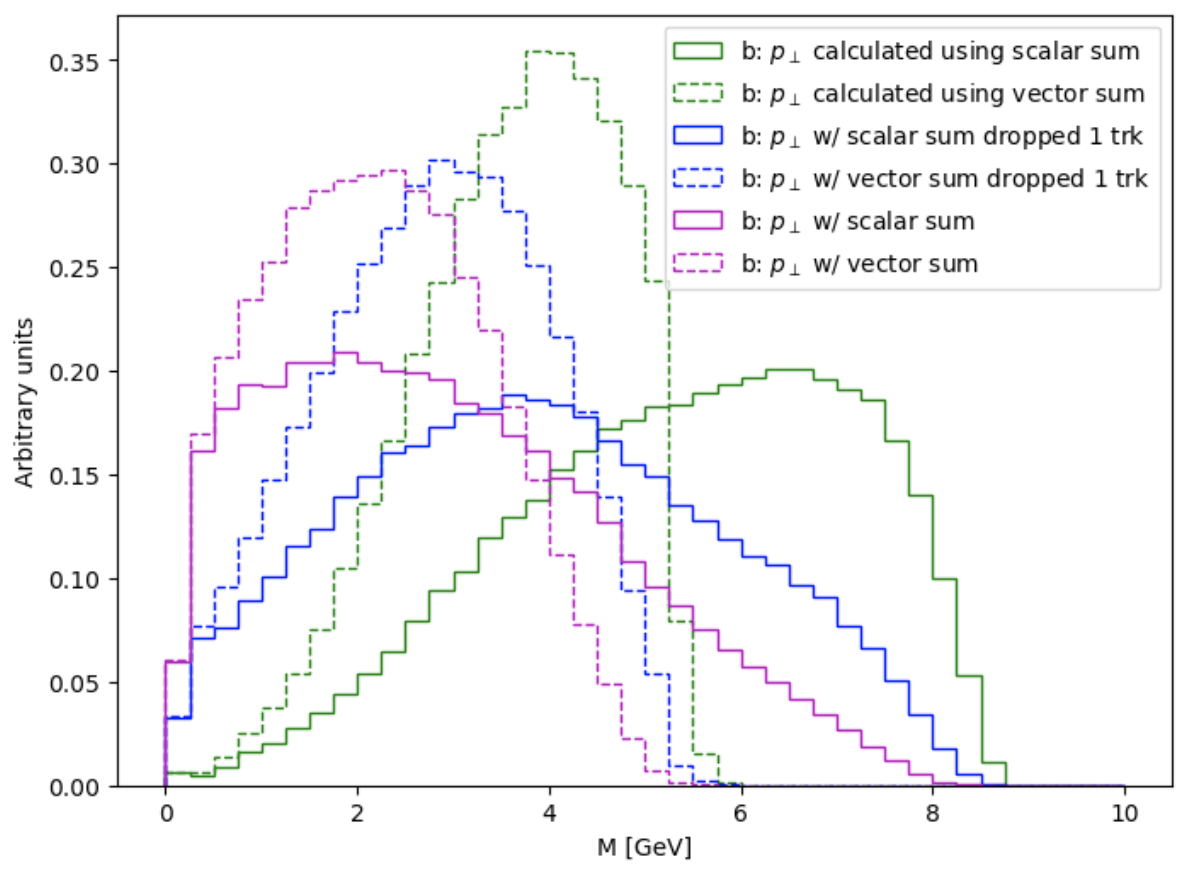
\includegraphics[width=0.45\textwidth]{{figures/ftag/mass-regression/b-had-drop-trks}}
	}
\subfloat[$D$-hadron reconstruction]{
	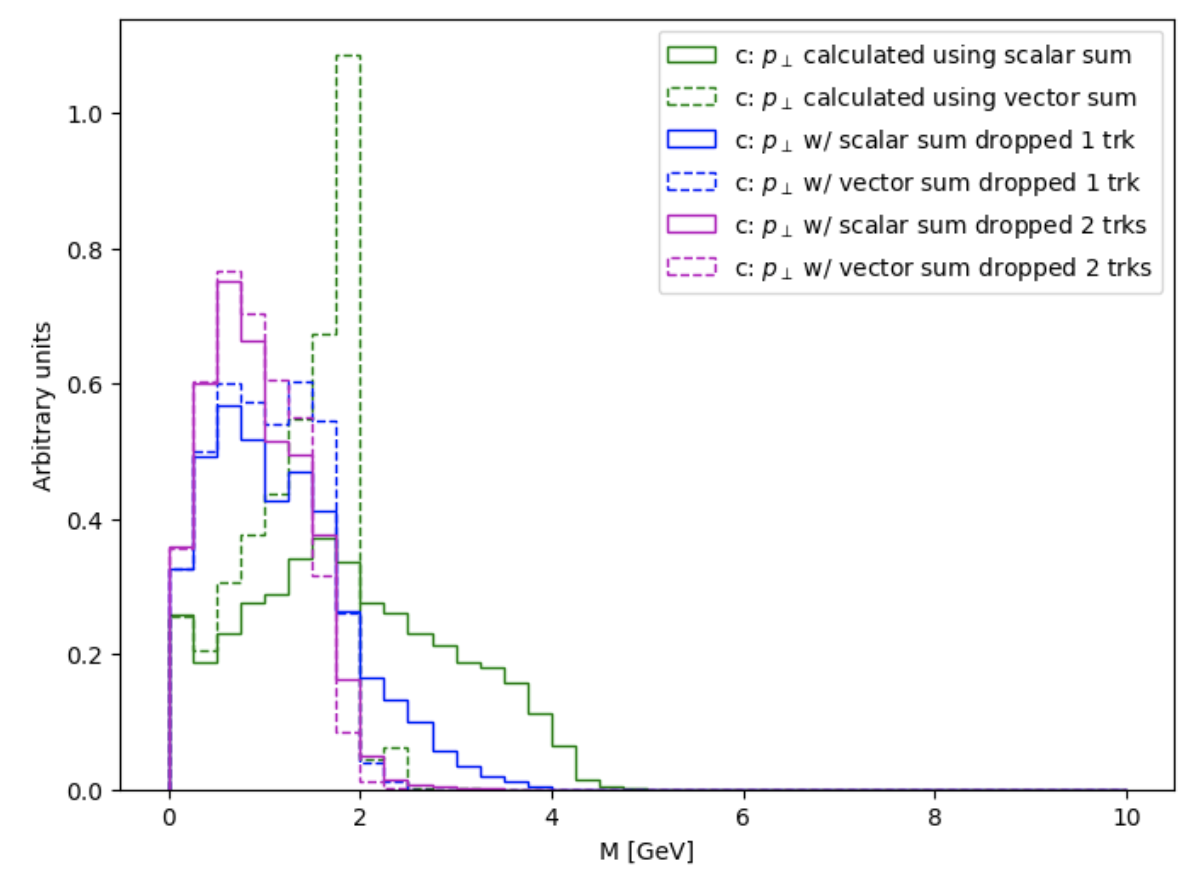
\includegraphics[width=0.45\textwidth]{{figures/ftag/mass-regression/c-had-drop-trks}}
	} \\
\subfloat[roc]{
	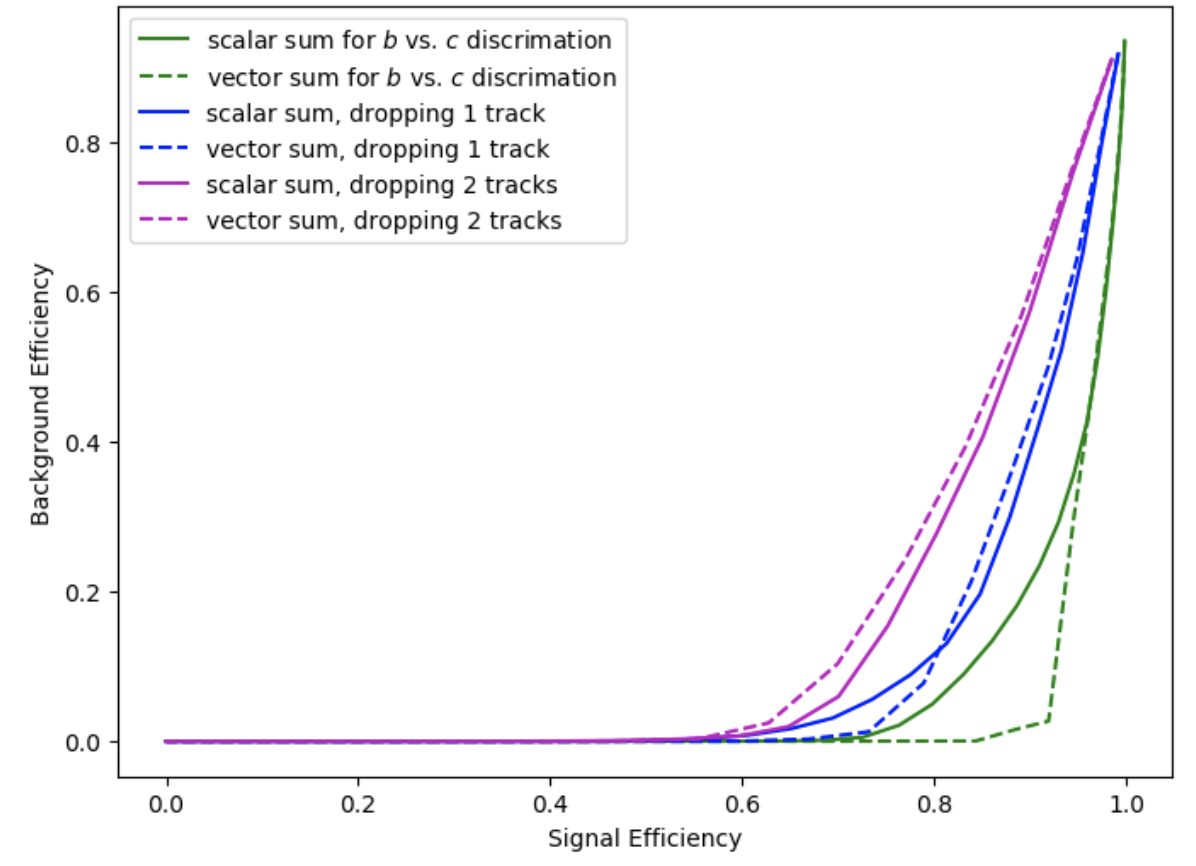
\includegraphics[width=0.7\textwidth]{{figures/ftag/mass-regression/roc-drop-trks}}
}
\caption{}%Reconstruction of the $B$ (left) and $D$ (right) hadron masses from the truth charged particles.}
\label{fig:truth-had-drop-trks}
\end{figure}


\begin{table}[h!]
\centering
\begin{tabular}{p{2cm} | p{12cm}  } 
\textbf{Input} & \textbf{Description}  \\
\hline
\hline
	 $m_{JF}$ & Invariant mass of the tracks attached to displaced vertices \\
	 $f_E$ & Fraction of the energy in the displaced vertices compared to the jet's energy \\
	 $\Delta R(\vec{p}_{jet}, \vec{p}_{vtx})$ & \\
	 $S_{xyz}$ & Average significance of all of the displaced vertices \\
	$n_{trk}$ & Number of tracks associated to the fitted displaced vertices along the cascade decay chain \\
	$n_{2-trk vtx}$ & Number of 2 track vertices (before the decay chain fit) \\
	$n_{1-trk vtx}$ & Number of the single track vertices (after the decay chain fit) \\
	$n_{\geq 2-trk vtx}$ & Number of the multi-prong displaced vertices (after the decay chain fit) \\
	\hline
	$L_{xyz}$(SV) & 3d distance from the first displaced vertex  \\
	$L_{xy}$(SV) &  transverse distance from the first displaced vertex \\
	$m_{trk}$(SV) & Mass of the tracks associated to the first displaced vertex \\
	$E_{trk}$(SV) & Energy of the tracks in the first displaced vertex \\
	$f_E$(SV) & Energy fraction of the tracks in the first displaced vertex compared to the energy of the jet \\ 
	$n_{vtx \ trk}$(SV) & Number of tracks attached to the first displaced vertex \\
\end{tabular}
\caption{Features from the JF reconstruction that are fed as input to the DL1r tagger. The first block of variables quantifies the global properties of the displaced vertices and decay topology. The second set of variables just looks at the properties of the first displaced vertex which capture the differences between \Pqb-jets and \Pqc-jets.}
\label{table:jf-inputs}
\end{table}


The jet input variables that (will be) shown in the FTAG algos paper:
\def\figpath{figures/ftag/ANA-FTAG-2019-07-PAPER/jetfitter}
\begin{figure}[htbp]
\centering
\subfloat[]{ 
    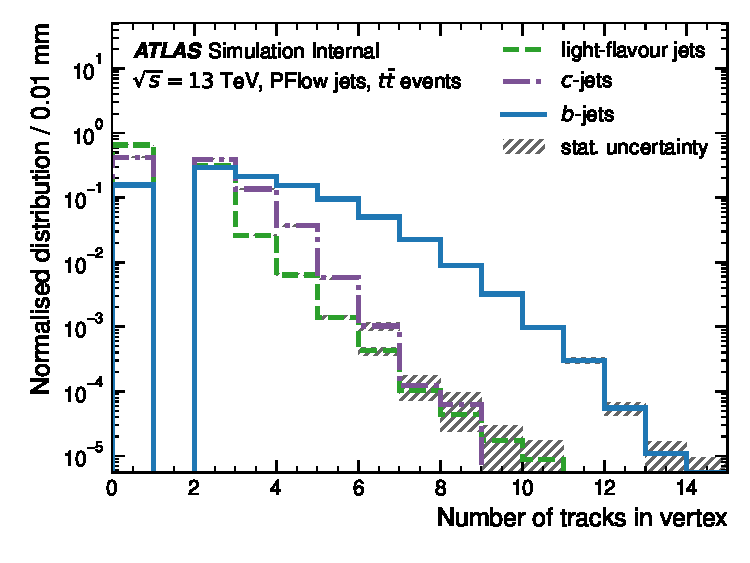
\includegraphics[width=0.32\linewidth]{\figpath/JetFitter_nTracksAtVtx_ttbar.pdf}
} 
\subfloat[]{ 
    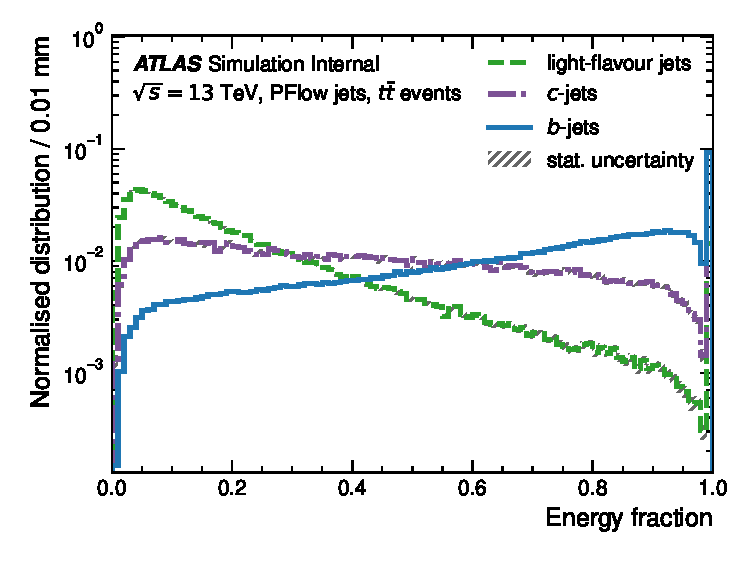
\includegraphics[width=0.32\linewidth]{\figpath/JetFitter_energyFraction_ttbar.pdf}
} 
     \subfloat[]{ 
    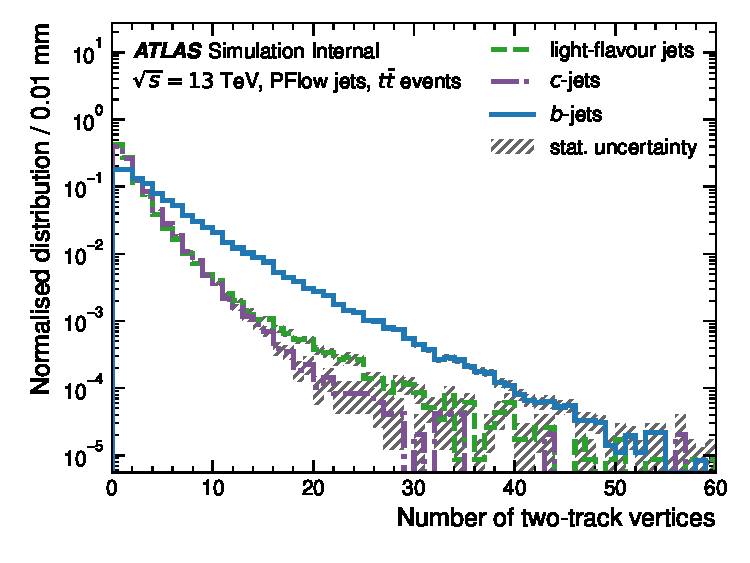
\includegraphics[width=0.32\linewidth]{\figpath/JetFitter_N2Tpair_ttbar.pdf}
} \\ 
\subfloat[]{ 
    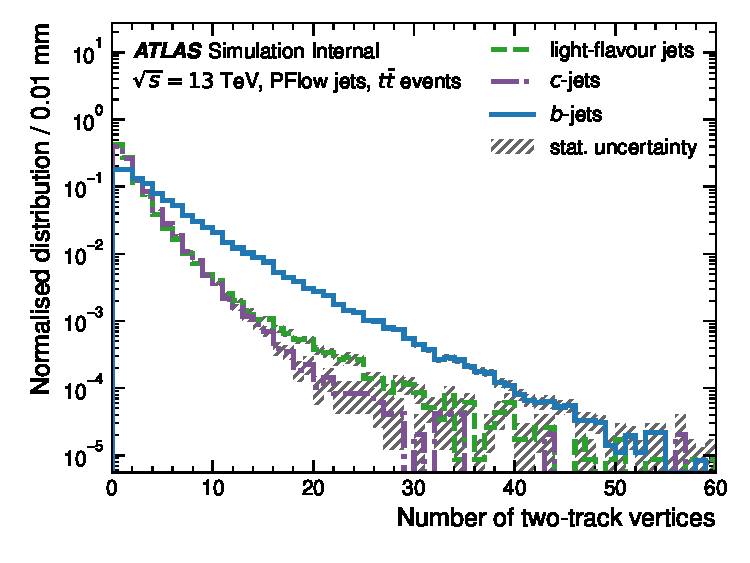
\includegraphics[width=0.32\linewidth]{\figpath/JetFitter_N2Tpair_ttbar.pdf}
} 
\subfloat[]{ 
    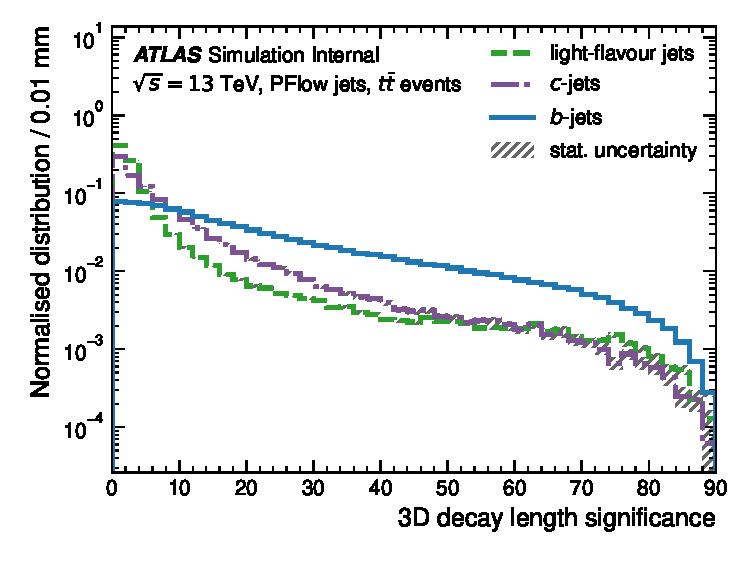
\includegraphics[width=0.32\linewidth]{\figpath/JetFitter_significance3d_ttbar.pdf}
} 
\subfloat[]{ 
    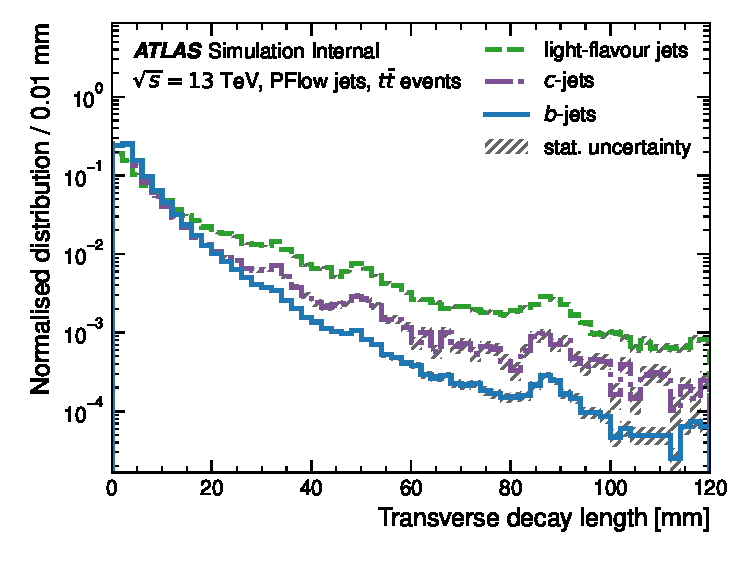
\includegraphics[width=0.32\linewidth]{\figpath/JetFitterSecondaryVertex_displacement2d_ttbar.pdf}
} 
\caption{The JF inputs that (will be) in the FTAG algos paper \cite{ANA-FTAG-2019-07}.}
\label{fig:sv1 inputs}
\end{figure}